\documentclass[12pt,a4paper]{article}
\usepackage{graphicx}
\usepackage{hyperref}
\title{Rosenblatt1958 — Research Booklet}
\date{}
\begin{document}
\maketitle
\tableofcontents
\newpage
\section{INFORMATION STORAGE AND ORGANIZATION}
Here is a summary of the section in clear, simple terms:

To understand how living things, like humans, can recognize things, remember, and think, we need to answer three very important questions.

Further reading: https://www.semanticscholar.org/search?q=INFORMATION%20STORAGE%20AND%20ORGANIZATION
\begin{figure}[h]
\centering
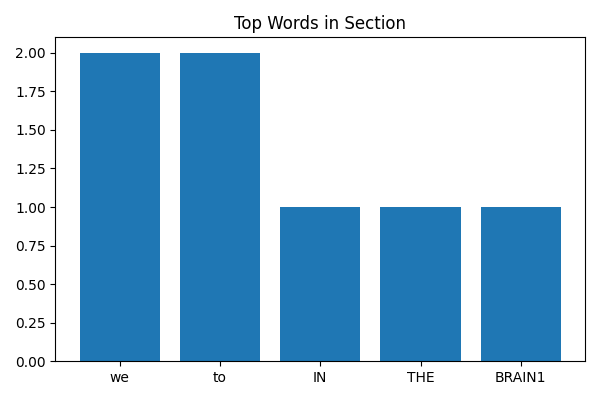
\includegraphics[width=0.8\textwidth]{D:\projects\mp 2 rag\autonomous rag\outputs\visual_5e0d43c7f4c54ffab230d70018fbd26f.png}
\end{figure}
\section{1. How is information about the}
Here is a summary of the section in clear, simple terms:

"How does our body detect or sense the world around us?"

Further reading: https://scholar.google.com/scholar?q=1.+How+is+information+about+the
\begin{figure}[h]
\centering
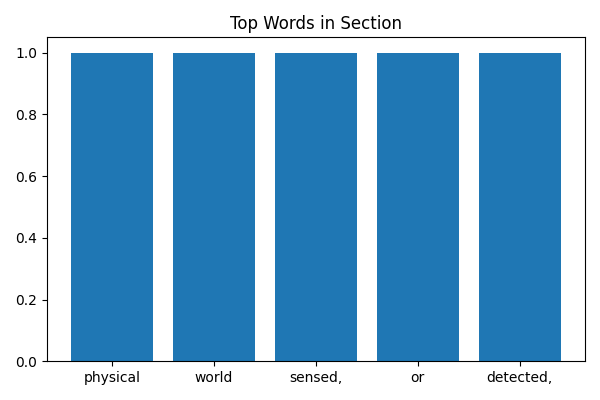
\includegraphics[width=0.8\textwidth]{D:\projects\mp 2 rag\autonomous rag\outputs\visual_de2c755528934881a59eff357d838303.png}
\end{figure}
\section{2. In what form is information}
I apologize, but you didn't provide a section for me to summarize. Please provide the text you'd like me to summarize, and I'll be happy to help!

Further reading: https://scholar.google.com/scholar?q=2.+In+what+form+is+information
\begin{figure}[h]
\centering
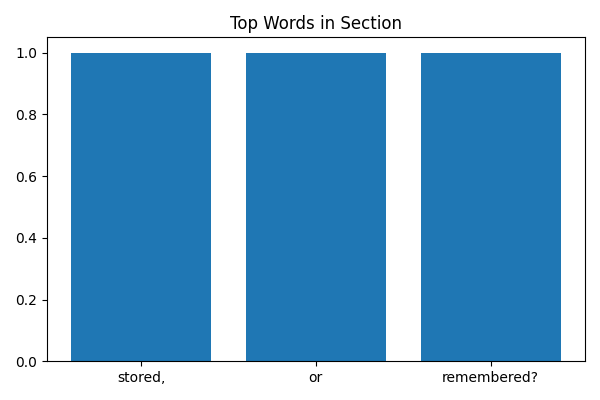
\includegraphics[width=0.8\textwidth]{D:\projects\mp 2 rag\autonomous rag\outputs\visual_9ffe4547f5dd43399b4a4142aad62cd9.png}
\end{figure}
\section{3. How does information contained}
Here's a summary of the section in clear and simple terms:

The article is discussing how our brains process and store information from our senses (like what we see and hear). There are three main questions about this:

1. How do our senses work? (This is the only question that scientists have a good understanding of.)
2. How do we store information from our senses in our brains?
3. How do we use that stored information to recognize things and behave in certain ways?

The article focuses on questions 2 and 3, which are still not well understood. There are two main ideas about how we store information:

Idea 1: Our brains store information as "coded representations" or "images" that can be reconstructed later, like a photograph.

Idea 2: Our brains don't store images at all, but instead create new connections between different parts of the brain when we learn something new. This means that there's no simple way to reconstruct the original information from our memories.

These two ideas are very different, and scientists are still trying to figure out which one is correct.

Further reading: https://www.semanticscholar.org/search?q=3.%20How%20does%20information%20contained
\begin{figure}[h]
\centering
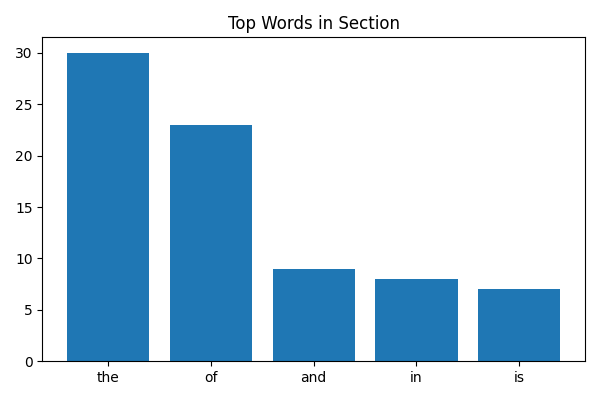
\includegraphics[width=0.8\textwidth]{D:\projects\mp 2 rag\autonomous rag\outputs\visual_39b2d3860ac24639be6dd13f893aceda.png}
\end{figure}
\section{THE PERCEPTRON}
Here's a simplified summary of the section:

**How does our brain store and use information?**

There are two main ideas about how our brain stores information:

1. **Coded memory**: Information is stored as a code, and when we see something, our brain compares it to the code to figure out what it is and how to respond.
2. **Connectionist**: Information is stored as connections between brain cells. When we see something, our brain uses these connections to automatically respond without needing to compare it to a code.

The author of this text supports the connectionist idea and has developed a theory called the "perceptron" to explain how it works.

**Background**

In the past, researchers have tried to understand how the brain works by creating models of how it might work. Some models are like computers, using logical rules to process information. Others are more like the brain, with many random connections between cells. However, these models have limitations and don't fully match how the brain actually works.

The author believes that a new approach is needed, one that uses probability theory to understand how the brain works. This approach is based on the idea that the brain is a complex system with many random connections, and that it can still work reliably despite these imperfections.

**Key points**

* The brain stores information as connections between cells, not as a code.
* When we see something, our brain uses these connections to respond automatically.
* The author has developed a theory called the "perceptron" to explain how this works.
* The perceptron is a model of how the brain might work, and it's based on probability theory rather than computer-like rules.

Further reading: https://scholar.google.com/scholar?q=THE+PERCEPTRON
\begin{figure}[h]
\centering
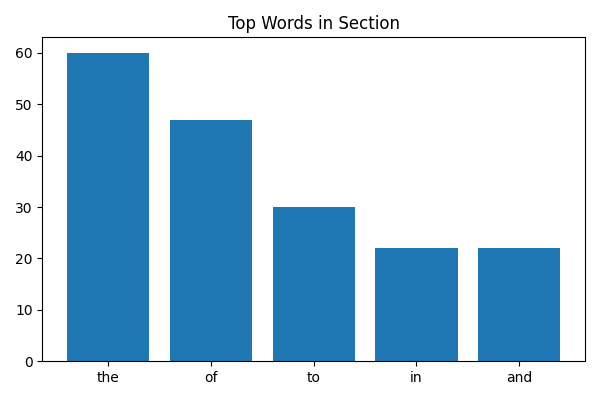
\includegraphics[width=0.8\textwidth]{D:\projects\mp 2 rag\autonomous rag\outputs\visual_9a3a8991739841828442749454c1b931.png}
\end{figure}
\section{1. The physical connections of the}
Here's a simple summary:

The parts of the brain that help us learn and recognize things are not exactly the same from one living thing to another. When we're born, the connections in our brain that are important for learning are mostly formed by chance, with only a few rules set by our genes.

Further reading: https://scholar.google.com/scholar?q=1.+The+physical+connections+of+the
\begin{figure}[h]
\centering
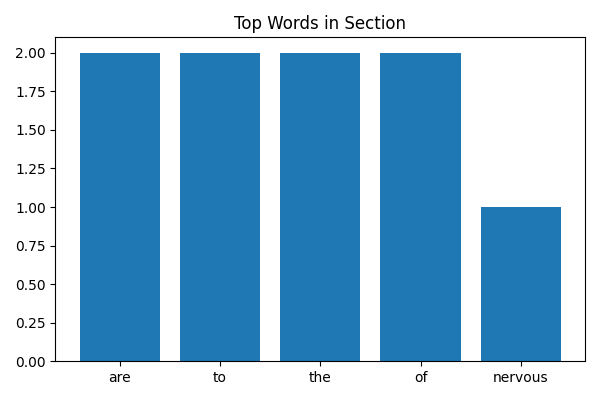
\includegraphics[width=0.8\textwidth]{D:\projects\mp 2 rag\autonomous rag\outputs\visual_e82ab67a5cfb48679926327ca1dcb803.png}
\end{figure}
\section{2. The original system of connected}
Here's a simple summary:

Brain cells can change and adapt over time. When some brain cells are active, it can affect how other brain cells respond to stimuli. This means that the connections between brain cells can get stronger or weaker based on what's happening in the brain.

Further reading: https://www.semanticscholar.org/search?q=2.%20The%20original%20system%20of%20connected
\begin{figure}[h]
\centering
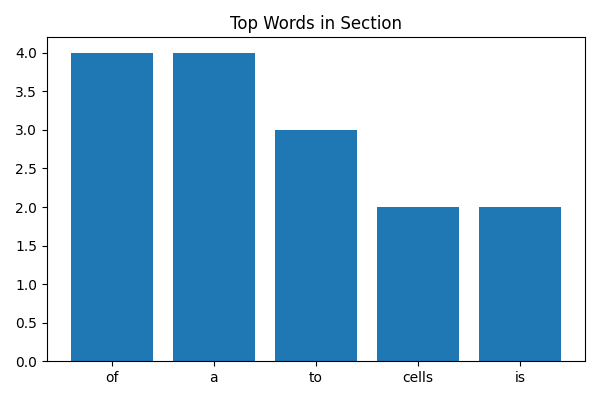
\includegraphics[width=0.8\textwidth]{D:\projects\mp 2 rag\autonomous rag\outputs\visual_3b8517b72cee43a49aa917520342a4ea.png}
\end{figure}
\section{3. Through exposure to a large}
Here's a simple summary:

The idea is that when looking at a group of things (like pictures or sounds), the ones that are most alike (in a way that makes sense for the specific situation) will tend to... (the sentence is incomplete, but this is the basic idea!)

Further reading: https://arxiv.org/search/?query=3.+Through+exposure+to+a+large&searchtype=all
\begin{figure}[h]
\centering
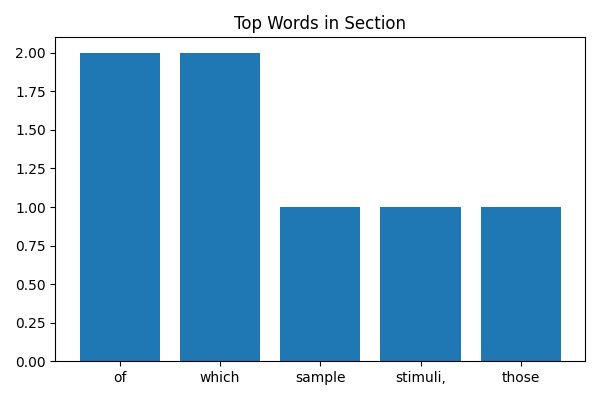
\includegraphics[width=0.8\textwidth]{D:\projects\mp 2 rag\autonomous rag\outputs\visual_21a5911a3173477e96836aaa1e0e3fcb.png}
\end{figure}
\section{THE PEECEPTRON}
Here's a simple summary:

Similar pathways will connect to the same group of cells, while very different pathways will connect to different groups of cells.

Further reading: https://scholar.google.com/scholar?q=THE+PEECEPTRON
\begin{figure}[h]
\centering
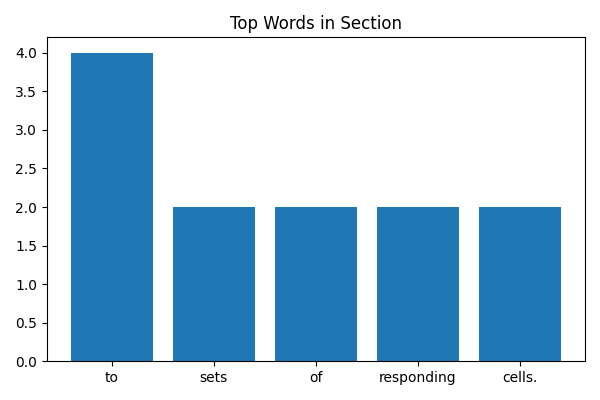
\includegraphics[width=0.8\textwidth]{D:\projects\mp 2 rag\autonomous rag\outputs\visual_2eeee16fffb34623aa0c847a88c1fb36.png}
\end{figure}
\section{4. The application of positive and/}
Here's a simple summary:

Rewards or punishments can help or hurt the process of learning and forming connections.

Further reading: https://arxiv.org/search/?query=4.+The+application+of+positive+and/&searchtype=all
\begin{figure}[h]
\centering
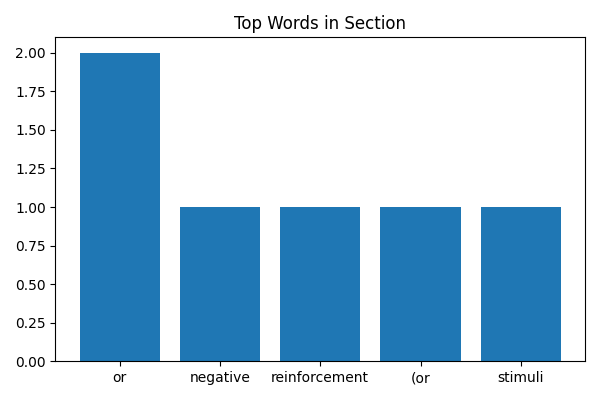
\includegraphics[width=0.8\textwidth]{D:\projects\mp 2 rag\autonomous rag\outputs\visual_68bd5926022547af884339b90d487d19.png}
\end{figure}
\section{5. Similarity, in such a system, is}
Here's a simple summary:

Our brains group similar things together because they trigger the same reactions in our nervous system. What makes things "similar" isn't about their shape or type, but about how our brains are organized and how we interact with the world around us. The way our brains are structured and the environment we're in will influence how we categorize and understand the world.

Further reading: https://www.semanticscholar.org/search?q=5.%20Similarity,%20in%20such%20a%20system,%20is
\begin{figure}[h]
\centering
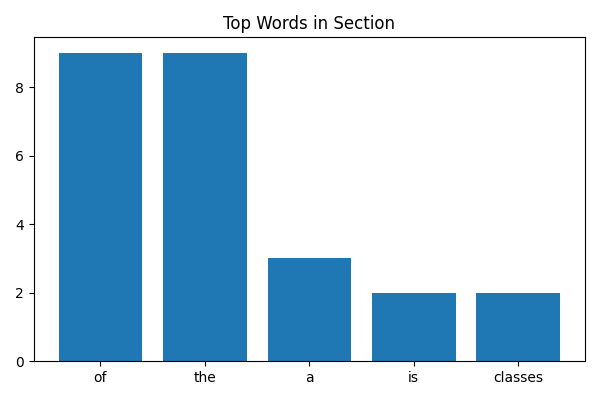
\includegraphics[width=0.8\textwidth]{D:\projects\mp 2 rag\autonomous rag\outputs\visual_85fa234d35764e339131569eeccaaed3.png}
\end{figure}
\section{THE ORGANIZATION OF A PERCEPTRON}
Here is a summary of the section in clear, simple terms:

A "photo-perceptron" is a special kind of computer system that can look at pictures and respond to what it sees. The way this system is organized is shown in a diagram called Fig. 1. There are certain rules that explain how this system is put together.

Further reading: https://www.semanticscholar.org/search?q=THE%20ORGANIZATION%20OF%20A%20PERCEPTRON
\begin{figure}[h]
\centering
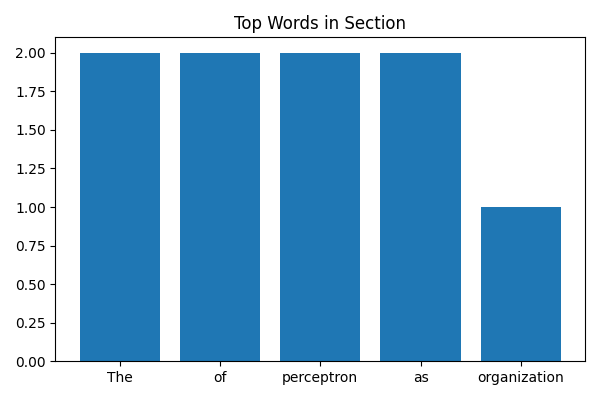
\includegraphics[width=0.8\textwidth]{D:\projects\mp 2 rag\autonomous rag\outputs\visual_54a85155da8d468591e017f585e5d855.png}
\end{figure}
\section{1. Stimuli impinge on a retina of}
Here's a simple summary:

Sensory units, also called S-points, are tiny parts that help us sense things. They can respond to stimuli (like light or sound) in different ways. In some models, they respond with a simple "yes" or "no" (all-or-nothing), while in others, they respond with a stronger or weaker signal depending on the strength of the stimulus. In this case, we're assuming they respond with a simple "yes" or "no".

Further reading: https://arxiv.org/search/?query=1.+Stimuli+impinge+on+a+retina+of&searchtype=all
\begin{figure}[h]
\centering
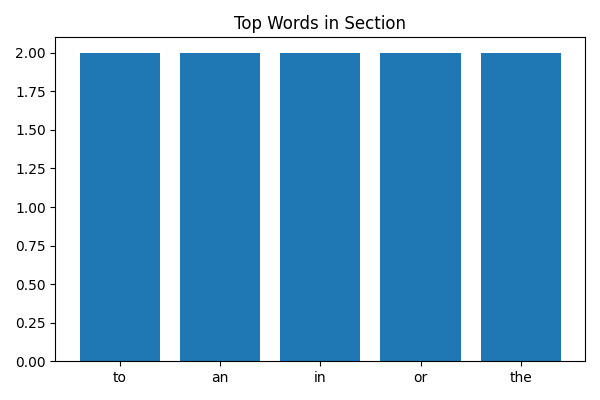
\includegraphics[width=0.8\textwidth]{D:\projects\mp 2 rag\autonomous rag\outputs\visual_ec8052e3c2b64764824402ae68e1131d.png}
\end{figure}
\section{2. Impulses are transmitted to a set}
Here's a simple summary:

Imagine a system that helps us understand how our brain processes visual information. This system has three parts: the retina (where light enters), a "projection area" (where the information is processed), and an "association area" (where the processed information is sent).

In the projection area, there are special cells called "A-units" that receive signals from the retina. Each A-unit gets signals from a specific group of points on the retina, called "origin points". These origin points can either excite or inhibit the A-unit, meaning they can either make it fire or not fire. If the total signal from the origin points is strong enough, the A-unit will fire.

The origin points for each A-unit are clustered together in a specific area of the retina, and the number of origin points decreases as you move further away from the center of that area. This helps our brain detect contours and shapes.

Further reading: https://arxiv.org/search/?query=2.+Impulses+are+transmitted+to+a+set&searchtype=all
\begin{figure}[h]
\centering
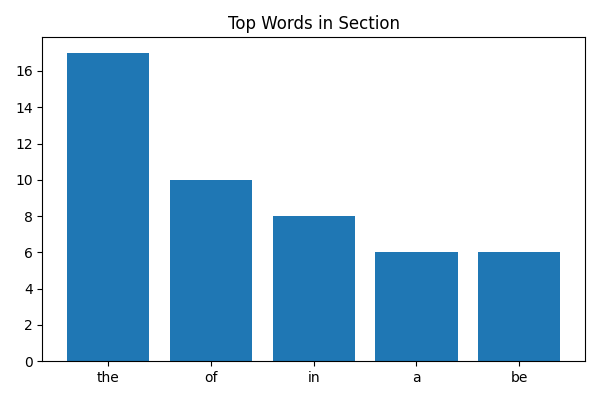
\includegraphics[width=0.8\textwidth]{D:\projects\mp 2 rag\autonomous rag\outputs\visual_b7bf440d288f497cbb87b7050b3dfc95.png}
\end{figure}
\section{3. Between the projection area and}
Here's a simple summary:

In the association area (An), the connections between units are random. This means that each unit in An gets connected to some units from another area (AI), but these connections are scattered randomly and not in a specific pattern. The units in An are similar to the units in AI and work in a similar way.

Further reading: https://arxiv.org/search/?query=3.+Between+the+projection+area+and&searchtype=all
\begin{figure}[h]
\centering
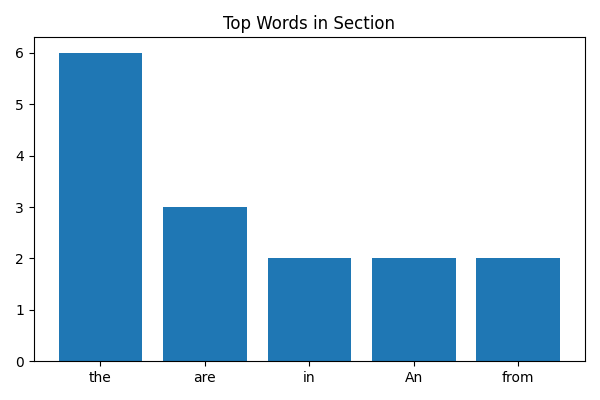
\includegraphics[width=0.8\textwidth]{D:\projects\mp 2 rag\autonomous rag\outputs\visual_e5b5198762a14e9da1069c20947afbbb.png}
\end{figure}
\section{4. The "responses," Ri, R^, . . . ,}
Here's a simple summary:

Imagine a network of cells that talk to each other. There are two types of cells: A-units and R-units. The A-units send signals to the R-units, and the R-units respond in a similar way to the A-units. Each R-unit response comes from a group of A-units that send signals to it, called the "source-set".

The signals travel from the A-units to the R-units in one direction, without any feedback loops. However, when the signals reach the R-units, they can send feedback signals back to the A-units. There are two ways this feedback can work:

1. The R-unit sends excitatory signals back to the A-units that sent signals to it, making them more active.
2. The R-unit sends inhibitory signals to the A-units that didn't send signals to it, making them less active.

The first option seems more likely based on how the brain is structured.

Further reading: https://scholar.google.com/scholar?q=4.+The+"responses,"+Ri,+R^,+.+.+.+,
\begin{figure}[h]
\centering
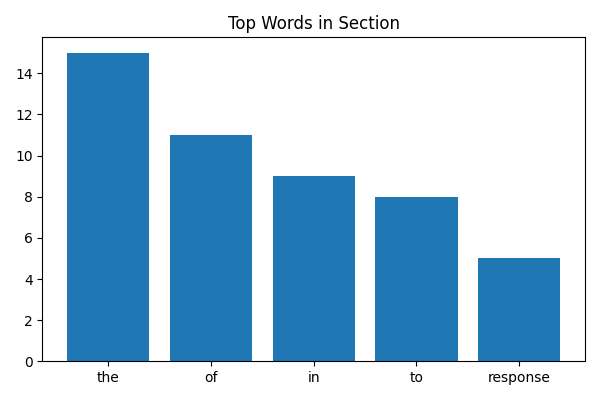
\includegraphics[width=0.8\textwidth]{D:\projects\mp 2 rag\autonomous rag\outputs\visual_c3d3ae6b1edf412cbdaba47a70084579.png}
\end{figure}
\section{COHKECTIOHI}
Here is a summary of the section in clear, simple terms:

Figure 2A shows a simple diagram of how a "perceptron" works. A perceptron is a type of artificial neural network. The diagram shows how different parts of the perceptron are connected to each other.

Further reading: https://www.semanticscholar.org/search?q=COHKECTIOHI
\begin{figure}[h]
\centering
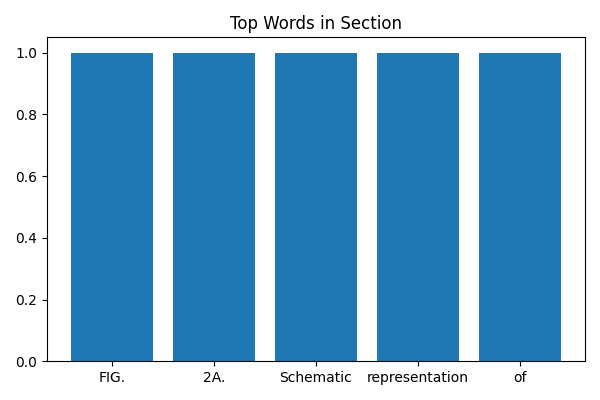
\includegraphics[width=0.8\textwidth]{D:\projects\mp 2 rag\autonomous rag\outputs\visual_5dc3cd272d8944349518132c9a35a605.png}
\end{figure}
\section{OWHWTMV OMNICTIOH}
Here's a summary of the section in clear and simple terms:

The section is talking about a type of artificial neural network called a perceptron. A perceptron is a system that helps computers learn and recognize patterns.

The diagram in Figure 2 shows a simplified version of a perceptron. This system has three stages and is connected in a special way that helps it recognize patterns based on similarities in the input data.

Each unit in the system has a random connection to the input data, which means it looks at different parts of the input data to recognize patterns. This system is good at recognizing patterns based on similarities, but not as good at recognizing patterns based on shapes or outlines.

The system can have multiple responses, but only one response can happen at a time. When one response happens, it blocks the other responses from happening. The response that happens is the one that gets the strongest or most frequent signal from the input data.

Overall, this system is a simple version of a perceptron that can help computers learn and recognize patterns in data.

Further reading: https://scholar.google.com/scholar?q=OWHWTMV+OMNICTIOH
\begin{figure}[h]
\centering
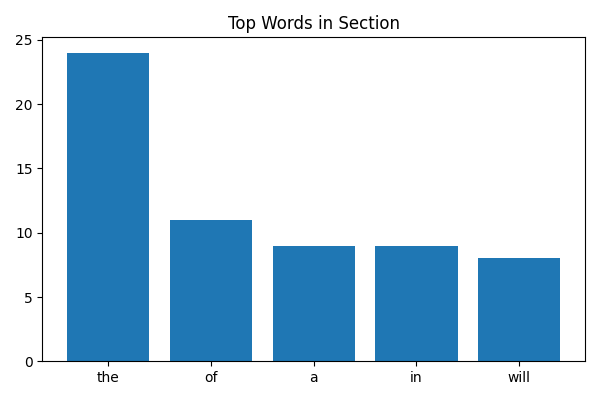
\includegraphics[width=0.8\textwidth]{D:\projects\mp 2 rag\autonomous rag\outputs\visual_d444dbb02209403fa81b3081227a7b96.png}
\end{figure}
\section{THE PERCEPTRON}
Here's a simplified summary of the section:

Imagine a system that can learn and respond to different stimuli. This system is made up of many small units called A-units, which can be connected to each other in different ways. When a stimulus is presented, some A-units respond and send signals to other units. The goal is to understand how the system learns to respond to different stimuli in a specific way.

The system has three types of rules for how the A-units change and learn:

1. Alpha system: When an A-unit is active, it gets a boost in strength that lasts forever.
2. Beta system: Each group of A-units gets a certain amount of strength, and the active units in the group share it.
3. Gamma system: When an A-unit is active, it takes strength away from the inactive units in its group, so the total strength of the group stays the same.

When a stimulus is presented, the system goes through two phases:

1. Predominant phase: Some A-units respond to the stimulus, but the system hasn't decided on a specific response yet.
2. Postdominant phase: One response becomes dominant and suppresses the other possible responses.

If the active A-units are "rewarded" (i.e., their strength is increased), they will be more likely to respond in the same way when the stimulus is presented again. This is how the system learns to respond to different stimuli in a specific way.

Further reading: https://www.semanticscholar.org/search?q=THE%20PERCEPTRON
\begin{figure}[h]
\centering
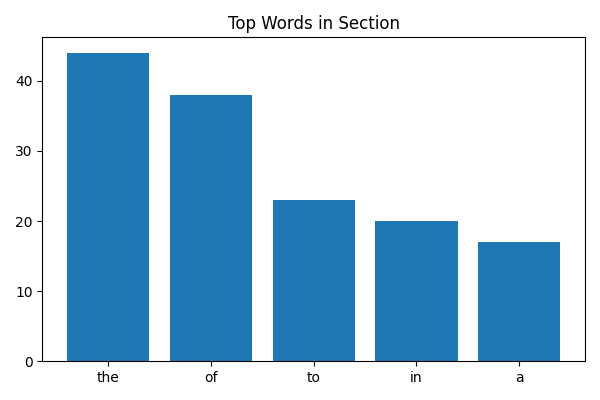
\includegraphics[width=0.8\textwidth]{D:\projects\mp 2 rag\autonomous rag\outputs\visual_1ef5cbb77850469ebd1801fdb904c672.png}
\end{figure}
\section{ANALYSIS OF THE PREDOMINANT
PHASE}
Here's a simple summary:

The perceptrons being discussed have a fixed threshold, meaning that the "A-units" (part of the perceptron) turn on or off based on a specific level of stimulation. This is different from a continuous model, where the response is gradual and depends on the strength of the stimulation.

To understand how these perceptrons learn, two important variables are considered:

1. Pa: the proportion of A-units that turn on when a stimulus of a certain size is applied.
2. Pc: the probability that an A-unit that responds to one stimulus will also respond to another similar stimulus.

As the size of the "retina" (the part of the perceptron that receives stimuli) increases, the number of stimuli points becomes less important, and the values of Pa and Pc approach what they would be if the retina were infinitely large. This means that the equations that describe the perceptron's behavior become simpler and more predictable.

Further reading: https://scholar.google.com/scholar?q=ANALYSIS+OF+THE+PREDOMINANT
PHASE
\begin{figure}[h]
\centering
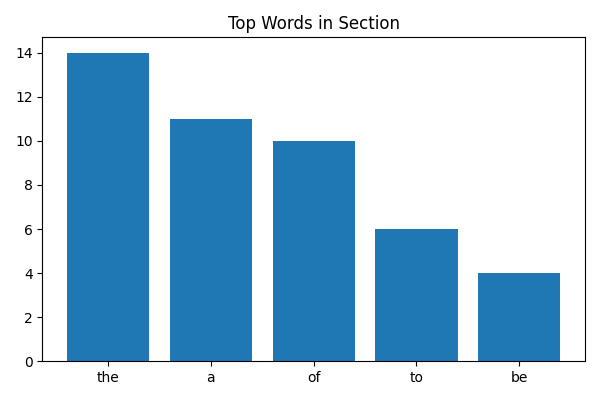
\includegraphics[width=0.8\textwidth]{D:\projects\mp 2 rag\autonomous rag\outputs\visual_ad198bf121e743138f308eb5008526be.png}
\end{figure}
\section{THE PERCEPTRON}
Here's a simple summary of the section:

This section is talking about how a certain type of unit (called an "A-unit") responds to a stimulus. The response depends on two things: how much the stimulus excites the unit (called "e") and how much it inhibits the unit (called "i").

The unit will respond if the total effect of the stimulus (e + i) is 6 or more.

The section also gives some math formulas to calculate the values of e and i, which depend on a few things:

* The number of connections that excite the unit (x)
* The number of connections that inhibit the unit (y)
* A threshold value (0) that determines how much stimulation is needed for the unit to respond
* A proportion of special points (called "S-points") that are activated by the stimulus (R)

The formulas are a bit complicated, but they help figure out how the unit will respond to the stimulus based on these different factors.

Further reading: https://arxiv.org/search/?query=THE+PERCEPTRON&searchtype=all
\begin{figure}[h]
\centering
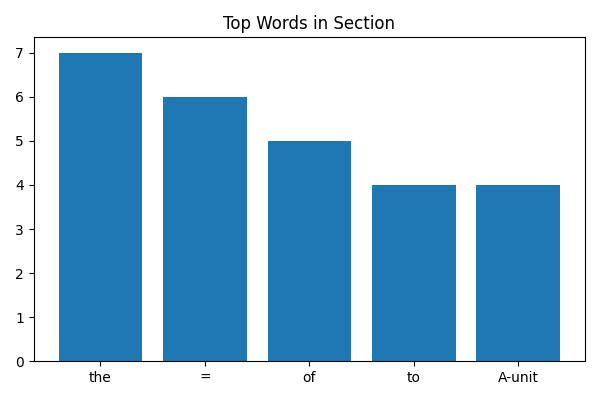
\includegraphics[width=0.8\textwidth]{D:\projects\mp 2 rag\autonomous rag\outputs\visual_d738b2032e024a6abfd6c89b304b06ec.png}
\end{figure}
\section{X
X}
Here's a summary of the section in clear and simple terms:

The section is talking about how two stimuli (S1 and S2) affect a unit called A-unit. The stimuli overlap on the retina, and the overlap is described by three quantities: R, L, and G.

* R is the proportion of the retina illuminated by both stimuli.
* L is the proportion of the retina illuminated by S1 but not S2.
* G is the proportion of the retina illuminated by S2 but not S1.

The section also talks about how the A-unit responds to the stimuli. It loses some excitatory and inhibitory points when S1 is replaced by S2, and gains some new ones. The response of the A-unit is affected by the threshold (δ) and the proportion of inhibitory connections (y).

The section shows some graphs that illustrate how the A-unit responds to different stimuli. The graphs show that:

* If the threshold is high or there are many inhibitory connections, the A-unit's response is reduced.
* If the excitation and inhibition are balanced, the A-unit's response is similar for stimuli of different sizes.
* The A-unit's response can be optimized by adjusting the threshold and inhibitory connections.

Overall, the section is discussing how the A-unit responds to different stimuli and how its response can be controlled and optimized.

Further reading: https://arxiv.org/search/?query=X
X&searchtype=all
\begin{figure}[h]
\centering
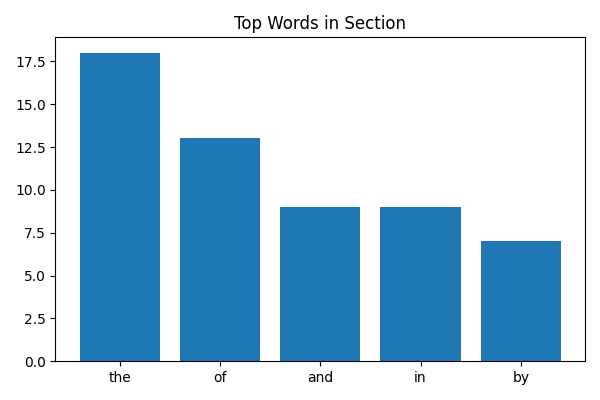
\includegraphics[width=0.8\textwidth]{D:\projects\mp 2 rag\autonomous rag\outputs\visual_3c7e0cf5d15d4151955baa222cd480fa.png}
\end{figure}
\section{4. Note that as the threshold is in-}
Here's a simple summary of the section:

The section is talking about how well a system can tell apart two different stimuli (like images). The system is made up of many small units that can be excited (turned on) or inhibited (turned off).

The researchers found that when there are more inhibitory connections, the system gets worse at telling apart the stimuli. They also found that even when the stimuli are completely different and don't overlap at all, the system can still tell them apart a little bit.

When the stimuli are similar, the system gets better at telling them apart. If the stimuli are very small or the system is very sensitive, it's harder for the system to tell them apart. But if the stimuli are very similar, the system can tell them apart very well.

This is important because it can help us understand how the system learns to tell apart different things.

Further reading: https://scholar.google.com/scholar?q=4.+Note+that+as+the+threshold+is+in-
\begin{figure}[h]
\centering
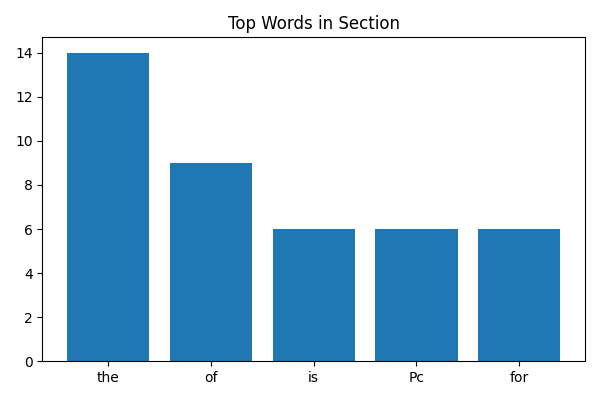
\includegraphics[width=0.8\textwidth]{D:\projects\mp 2 rag\autonomous rag\outputs\visual_7b6afd32cb684b7392542e0334a3d214.png}
\end{figure}
\section{MATHEMATICAL ANALYSIS
OF LEARNING IN THE
PERCEPTRON}
Here's a simple summary:

When a perceptron (a type of artificial neural network) is given a stimulus, it first responds with many units reacting. But soon, only one group of units remains active, while the others are suppressed. There are two ways this "winner" group is determined:

1. The "mean-discriminating system" chooses the group with the highest average input value.
2. The "sum-discriminating system" chooses the group with the highest total input value.

In most cases, the first system (mean-discriminating) works better than the second system (sum-discriminating).

Further reading: https://www.semanticscholar.org/search?q=MATHEMATICAL%20ANALYSIS
OF%20LEARNING%20IN%20THE
PERCEPTRON
\begin{figure}[h]
\centering
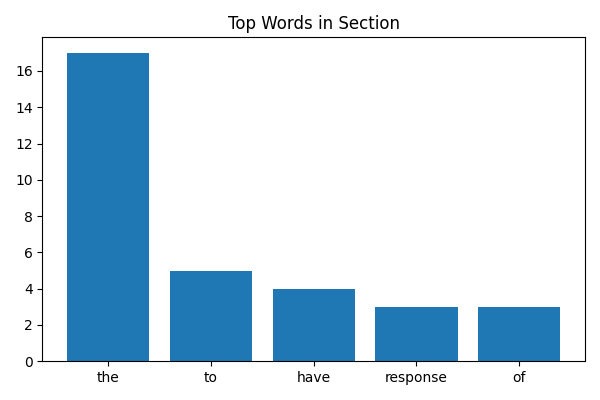
\includegraphics[width=0.8\textwidth]{D:\projects\mp 2 rag\autonomous rag\outputs\visual_42e1de8104b84e748cdf1519a96ad717.png}
\end{figure}
\section{THE PERCEPTEON}
Here's a simplified summary of the section:

The section discusses how a perceptron (a type of artificial neural network) learns and makes decisions. The perceptron is shown a series of stimuli, and it's forced to respond in a certain way. Then, it's tested to see how well it remembers the correct responses.

There are two types of experiments:

1. The perceptron is shown the same stimuli again, and its ability to recall the correct responses is measured (called Pr).
2. The perceptron is shown new stimuli that are similar to the ones it learned from, but not exactly the same. Its ability to generalize and respond correctly to these new stimuli is measured (called Pg).

The section introduces a mathematical equation that describes how well the perceptron performs in these experiments. The equation takes into account the number of "effective" units in the perceptron that are involved in making decisions, as well as the characteristics of the stimuli and the environment in which the perceptron is learning.

The simplest case to analyze is when the perceptron is shown random, unclassified stimuli, and its performance is measured in this "ideal" environment.

Further reading: https://www.semanticscholar.org/search?q=THE%20PERCEPTEON
\begin{figure}[h]
\centering
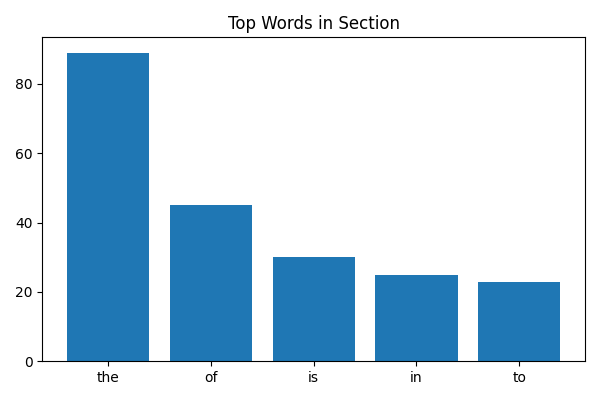
\includegraphics[width=0.8\textwidth]{D:\projects\mp 2 rag\autonomous rag\outputs\visual_0d462f0c50ef485cb5b769730c47e99d.png}
\end{figure}
\section{THE PERCEPTRON}
Here's a summary of the section in clear and simple terms:

The section discusses three systems (alpha, beta, and gamma) that learn from experiences. These systems try to predict the best response to a stimulus. The goal is to understand how well each system performs.

In the alpha system, each response is associated with a certain number of stimuli. If this number is fixed, the system performs well. But if the number of stimuli varies randomly, the system's performance is poorer.

The beta system performs even worse than the alpha system because it amplifies small differences, leading to unreliable results.

The gamma system is different from the other two. It doesn't matter which method it uses to make predictions, and its performance is not affected by the variability in the number of stimuli associated with each response.

The section also presents some mathematical equations and graphs to illustrate the performance of each system under different conditions.

Further reading: https://scholar.google.com/scholar?q=THE+PERCEPTRON
\begin{figure}[h]
\centering
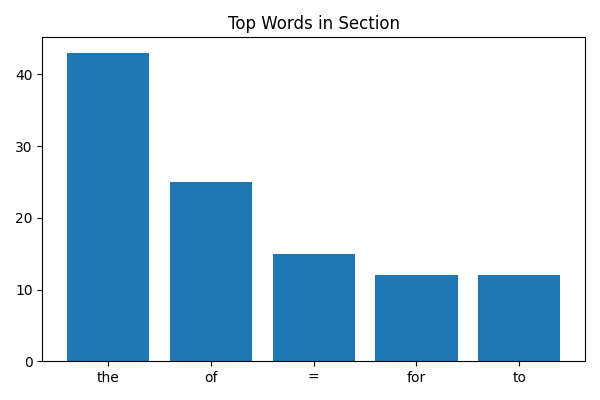
\includegraphics[width=0.8\textwidth]{D:\projects\mp 2 rag\autonomous rag\outputs\visual_63abcd1788664c4583091bd6c9174826.png}
\end{figure}
\section{THE PERCEPTRON}
Here's a summary of the section in clear, simple terms:

The section compares the performance of three systems (α, β, and 7) in different environments. In an "ideal" environment, the systems perform similarly. However, in a "differentiated" environment, where there are different classes of stimuli (e.g., squares, circles, and triangles), the systems perform differently.

In a differentiated environment, the perceptron (a type of system) learns to generalize well, meaning it can correctly respond to new stimuli it hasn't seen before. This is because the perceptron can learn to recognize patterns within each class of stimuli.

The section also introduces a new concept called PCap, which measures the performance of the system in a differentiated environment. PCap is the expected value of the probability of correct generalization between pairs of stimuli drawn from different classes.

The section concludes by showing that, in a differentiated environment, the perceptron can learn to generalize well if the parameters of the system are properly chosen. This means that the perceptron can learn to respond correctly to new stimuli, even if it hasn't seen them before, as long as they belong to a class of stimuli it has learned to recognize.

Further reading: https://arxiv.org/search/?query=THE+PERCEPTRON&searchtype=all
\begin{figure}[h]
\centering
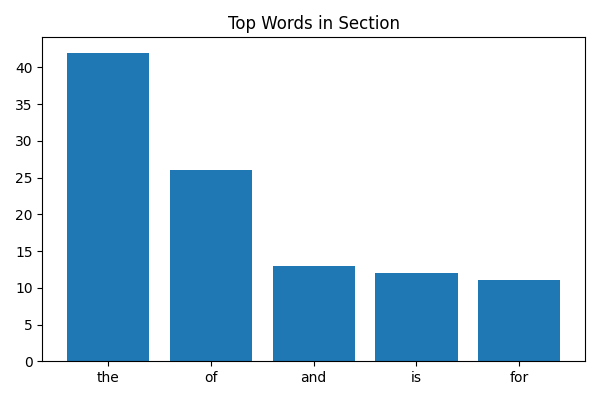
\includegraphics[width=0.8\textwidth]{D:\projects\mp 2 rag\autonomous rag\outputs\visual_8335da6ef35942e496dbf9ed429d3670.png}
\end{figure}
\section{THE PERCEPTSON}
Here's a summary of the section in clear and simple terms:

The section is talking about a mathematical model that tries to understand how our brain learns to recognize and distinguish between different stimuli (like shapes or objects). The model uses some complex equations to calculate how well the brain can learn to recognize these stimuli.

The equations involve some variables that are hard to analyze precisely, so they are treated as unknown values that need to be determined through experimentation. The model assumes that some of these variables are very small and can be ignored.

The section also talks about how the brain's performance in recognizing stimuli improves as it gets more practice and experience. However, if the brain has to recognize too many different stimuli, its performance gets worse unless it uses a special way of coding the information called "binary coding". This coding method helps the brain to recognize stimuli more efficiently by breaking them down into simpler features.

For example, instead of trying to recognize 100 different objects, the brain can recognize a few simple features like "dark" or "light", "tall" or "short", and so on. This way, the brain can distinguish between many different stimuli using just a few simple features.

Further reading: https://arxiv.org/search/?query=THE+PERCEPTSON&searchtype=all
\begin{figure}[h]
\centering
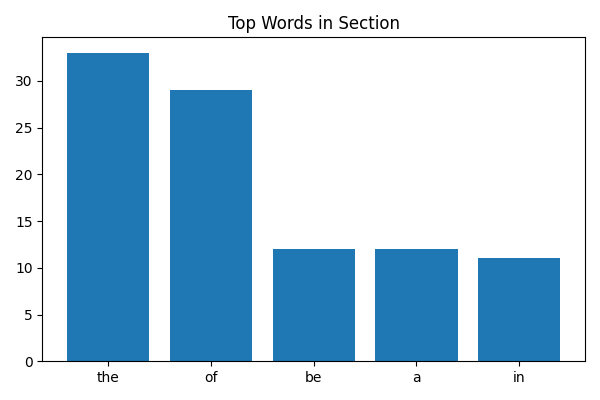
\includegraphics[width=0.8\textwidth]{D:\projects\mp 2 rag\autonomous rag\outputs\visual_2adf36c2d589467faead2ba47362c810.png}
\end{figure}
\section{BIVALENT SYSTEMS}
Here's a simple summary:

In some systems, when a unit is active and gets reinforced, it always gets stronger and better at doing its job. But in a special kind of system called a "bivalent system", an active unit can either get stronger or weaker, depending on what's happening in the system. This is like a system that can use rewards and punishments to teach it new things. But even if there are no rewards or punishments, a bivalent system can still work by using positive and negative feedback to help it learn.

Further reading: https://scholar.google.com/scholar?q=BIVALENT+SYSTEMS
\begin{figure}[h]
\centering
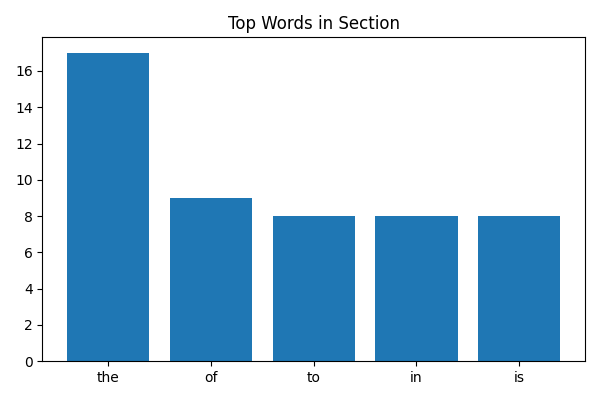
\includegraphics[width=0.8\textwidth]{D:\projects\mp 2 rag\autonomous rag\outputs\visual_b0f98b9718f749f7a6a974dd9de50aa6.png}
\end{figure}
\section{THE PERCEPTRON}
Here's a summary of the section in clear and simple terms:

This section talks about a type of system that helps reduce biases in decision-making. Biases happen when we prefer one answer over another because of things like size or frequency. This system is called a "bivalent system".

In this system, when we get a reward (positive reinforcement), it adds a positive value to the "on" responses and a negative value to the "off" responses. When we get a punishment (negative reinforcement), it does the opposite.

This system works well because it can help us make correct decisions even when there are biases. The system can be made more realistic by adding "excitatory" and "inhibitory" units that work together to make decisions.

Computer simulations have been done to test this system, and the results match the theory. This means that the system works as expected and can help reduce biases in decision-making.

Further reading: https://www.semanticscholar.org/search?q=THE%20PERCEPTRON
\begin{figure}[h]
\centering
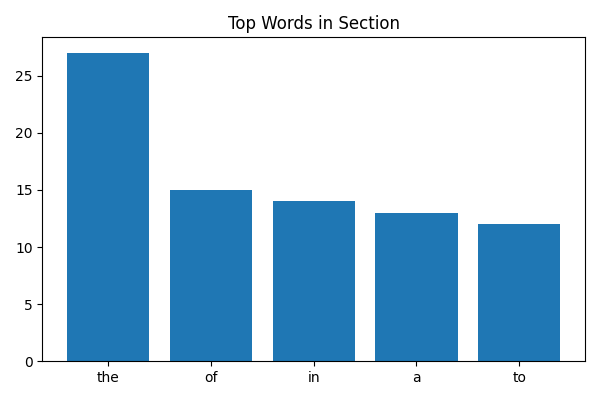
\includegraphics[width=0.8\textwidth]{D:\projects\mp 2 rag\autonomous rag\outputs\visual_fe1a27bf55fc4098a9c281038444e87f.png}
\end{figure}
\section{IMPROVED PERCEPTRONS AND
SPONTANEOUS ORGANIZATION}
Here's a summary of the section in clear and simple terms:

The previous sections talked about how a perceptron (a type of artificial neural network) can recognize patterns, but didn't consider time as a factor. However, it's possible to make a perceptron that can recognize patterns that change over time, like velocities or sound sequences.

The perceptron can also be designed to be sensitive to the location of contours, and can even form concepts on its own when exposed to random stimuli. This means it can learn to recognize the difference between two classes of stimuli without being told what's right or wrong.

The perceptron can also be used for selective recall and attention, and can associate sounds with visual objects. It can even perform tasks like naming objects or colors when given a command.

The question is, how far can the perceptron's capabilities go? It can do pattern recognition, learning, and attention, and can even learn to recognize temporal patterns. However, it's limited in its ability to make relative judgments and understand relationships between stimuli. It can learn to respond to concrete stimuli, but struggles with more abstract tasks that require understanding relationships between things.

Further reading: https://arxiv.org/search/?query=IMPROVED+PERCEPTRONS+AND
SPONTANEOUS+ORGANIZATION&searchtype=all
\begin{figure}[h]
\centering
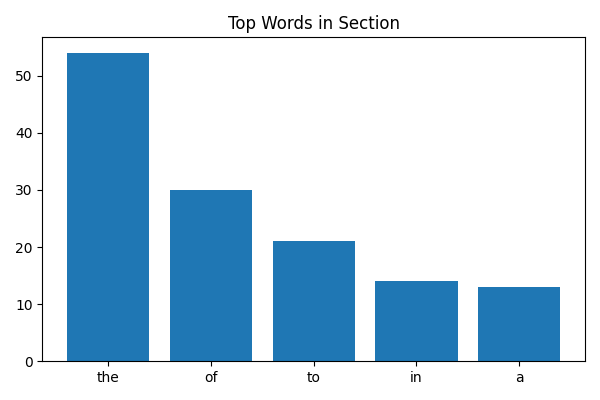
\includegraphics[width=0.8\textwidth]{D:\projects\mp 2 rag\autonomous rag\outputs\visual_e6e301fa178c47c2a6e36e291f14f2bd.png}
\end{figure}
\section{THE PESCEPTRON}
Here's a simple summary:

When trying to solve a complex problem using a perceptron (a type of artificial neural network), it becomes too hard to solve. Just being able to separate data into different groups (statistical separability) isn't enough to handle more complex thinking. A more advanced system is needed to tackle these kinds of problems.

Further reading: https://scholar.google.com/scholar?q=THE+PESCEPTRON
\begin{figure}[h]
\centering
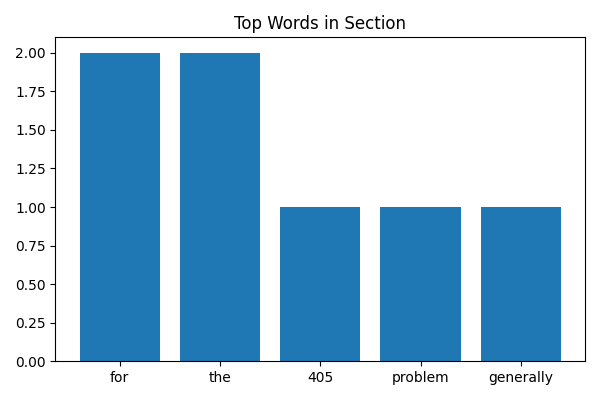
\includegraphics[width=0.8\textwidth]{D:\projects\mp 2 rag\autonomous rag\outputs\visual_478adf728a374687839c3a765969e596.png}
\end{figure}
\section{CONCLUSIONS AND EVALUATION}
Here is a summary of the section in clear, simple terms:

The main points from studying the perceptron are:

Further reading: https://arxiv.org/search/?query=CONCLUSIONS+AND+EVALUATION&searchtype=all
\begin{figure}[h]
\centering
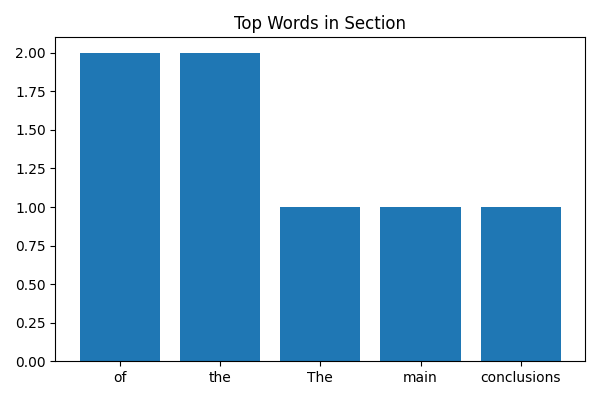
\includegraphics[width=0.8\textwidth]{D:\projects\mp 2 rag\autonomous rag\outputs\visual_8a11ef9f21b245bf94a4c041c907a79f.png}
\end{figure}
\section{1. In an environment of random}
Here's a simple summary:

A system made up of many connected parts can learn to respond in specific ways to specific things it senses (like sights or sounds). Even if many of these things are similar and trigger similar reactions, the system can still recognize them correctly more often than not.

Further reading: https://scholar.google.com/scholar?q=1.+In+an+environment+of+random
\begin{figure}[h]
\centering
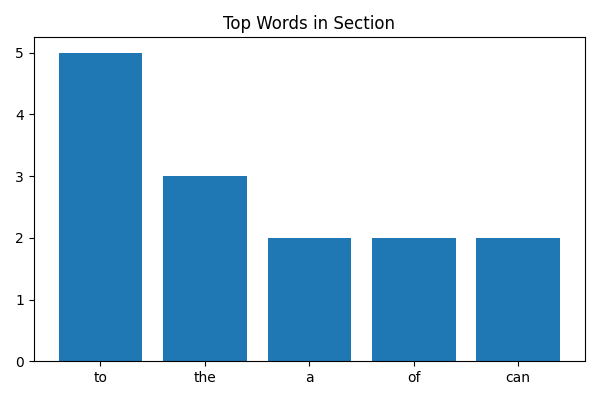
\includegraphics[width=0.8\textwidth]{D:\projects\mp 2 rag\autonomous rag\outputs\visual_d8b6556240cb4932ae88e06e75369547.png}
\end{figure}
\section{2. In such an "ideal environment,"}
As you learn more things, it becomes harder to remember them correctly. Eventually, your ability to recall them correctly goes back down to the same level as if you had never learned them at all.

Further reading: https://www.semanticscholar.org/search?q=2.%20In%20such%20an%20"ideal%20environment,"
\begin{figure}[h]
\centering
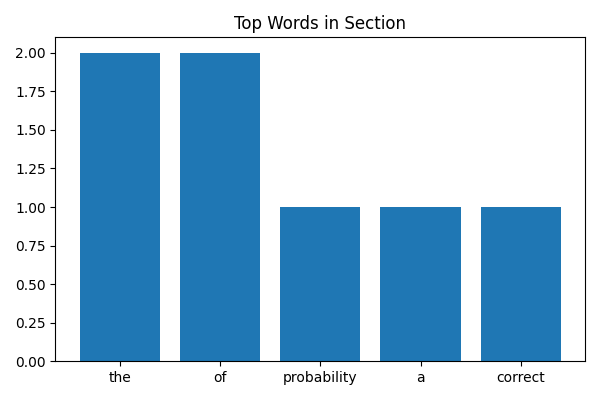
\includegraphics[width=0.8\textwidth]{D:\projects\mp 2 rag\autonomous rag\outputs\visual_40f7e46613574a0a9ef6a0f449e324ea.png}
\end{figure}
\section{3. In such an environment, no basis}
I apologize, but the section you provided is incomplete and doesn't make sense on its own. It seems like a sentence fragment.

Could you please provide more context or complete the sentence so I can help you summarize it in clear and simple terms?

Further reading: https://arxiv.org/search/?query=3.+In+such+an+environment,+no+basis&searchtype=all
\begin{figure}[h]
\centering
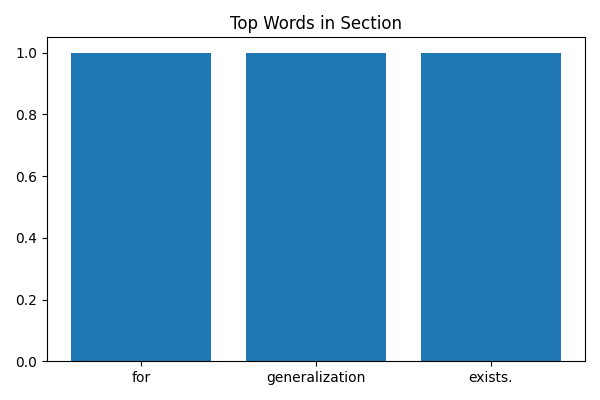
\includegraphics[width=0.8\textwidth]{D:\projects\mp 2 rag\autonomous rag\outputs\visual_18a58eae55eb4b9298631a3febf7fe5e.png}
\end{figure}
\section{4. In a "differentiated environ-}
Here's a simple summary:

When a system learns to associate different stimuli with specific responses, it gets better at remembering the correct associations as it learns more stimuli. The more it learns, the closer it gets to being perfect. And, if you add more "association cells" to the system, it can get almost 100% accurate.

Further reading: https://arxiv.org/search/?query=4.+In+a+"differentiated+environ-&searchtype=all
\begin{figure}[h]
\centering
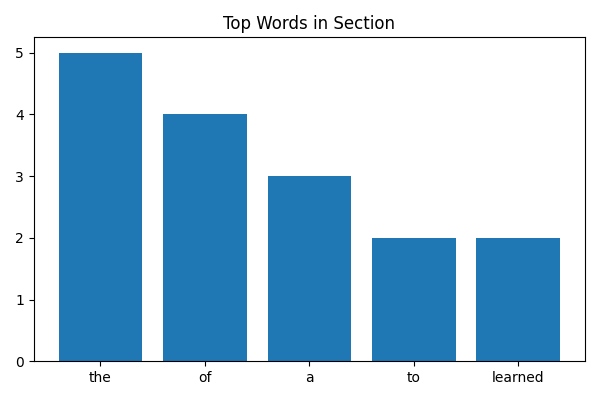
\includegraphics[width=0.8\textwidth]{D:\projects\mp 2 rag\autonomous rag\outputs\visual_bca06e8135554a26b9b96a5e0b776ac2.png}
\end{figure}
\section{5. In the differentiated environ-}
Here's a simple summary:

When you show someone a new thing they've never seen before, they have a certain chance of correctly identifying what it is and grouping it with similar things. As they get more experience, this chance of correct identification gets closer to the chance of correctly identifying something they've seen before. This will happen if certain conditions are met, and it will be better than just guessing.

Further reading: https://arxiv.org/search/?query=5.+In+the+differentiated+environ-&searchtype=all
\begin{figure}[h]
\centering
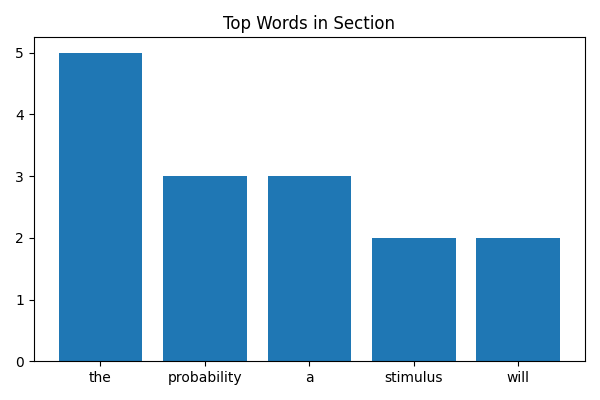
\includegraphics[width=0.8\textwidth]{D:\projects\mp 2 rag\autonomous rag\outputs\visual_4565a1dbc578432db3f8c32c49fd1901.png}
\end{figure}
\section{6. The performance of the system}
Here's a summary of the section in simple terms:

To make things better, you can:

1. Use a special way of showing information that pays attention to the outlines or shapes of things.
2. Use a system where each answer (or "bit") corresponds to a specific feature or characteristic of what you're looking at.

Further reading: https://www.semanticscholar.org/search?q=6.%20The%20performance%20of%20the%20system
\begin{figure}[h]
\centering
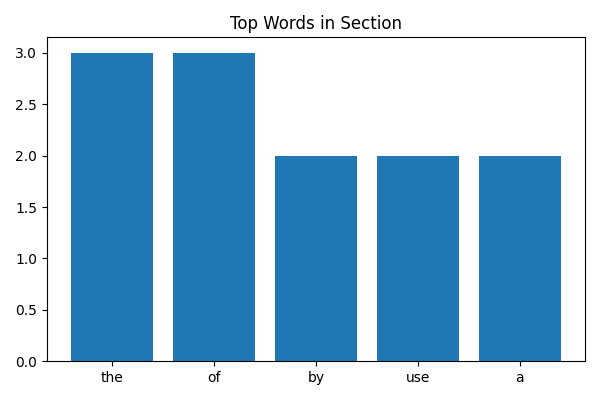
\includegraphics[width=0.8\textwidth]{D:\projects\mp 2 rag\autonomous rag\outputs\visual_762b06dedcb845868dd997b20015e751.png}
\end{figure}
\section{7. Trial-and-error learning is possi-}
I apologize, but the text "ble in bivalent reinforcement systems" doesn't make sense and appears to be incomplete or contain a typo. Could you please provide more context or clarify what you mean by this phrase?

If you meant to ask about "able in bivalent reinforcement systems", I'd be happy to help. Bivalent reinforcement systems refer to a type of learning process where an individual receives both rewards and punishments for their behavior. In this context, being "able" in such systems would mean that an individual is capable of learning and adapting to the consequences of their actions, despite the mixed signals they receive.

Further reading: https://arxiv.org/search/?query=7.+Trial-and-error+learning+is+possi-&searchtype=all
\begin{figure}[h]
\centering
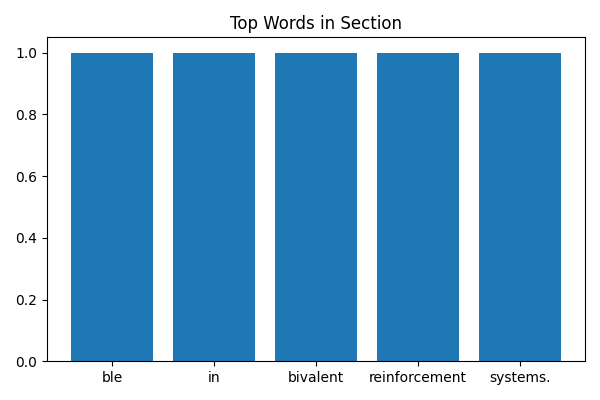
\includegraphics[width=0.8\textwidth]{D:\projects\mp 2 rag\autonomous rag\outputs\visual_d5a196925b30410cac5d01c233981df8.png}
\end{figure}
\section{8. Temporal organizations of both}
Here's a simple summary:

A system can learn to recognize patterns and respond to them by building on its existing abilities, without needing to become more complex.

Further reading: https://arxiv.org/search/?query=8.+Temporal+organizations+of+both&searchtype=all
\begin{figure}[h]
\centering
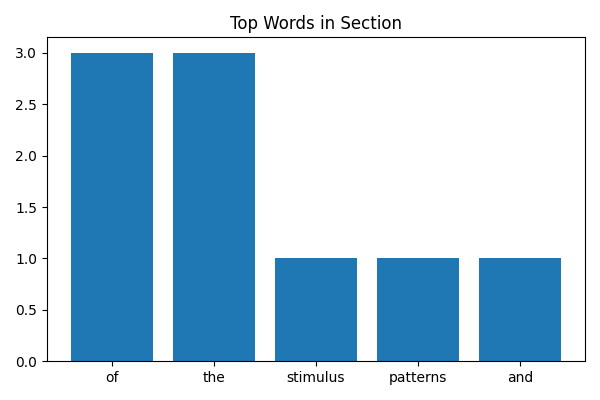
\includegraphics[width=0.8\textwidth]{D:\projects\mp 2 rag\autonomous rag\outputs\visual_bce05b2cf6e04235bc79b782c53a6f00.png}
\end{figure}
\section{9. The memory of the perceptron}
Here's a simple summary:

The association system in the brain is spread out and shared. This means that many different connections can use the same "cells" (or brain areas). If some of these cells are damaged or removed, it won't greatly affect any one specific memory or skill. However, it will start to cause problems with many learned associations overall.

Further reading: https://www.semanticscholar.org/search?q=9.%20The%20memory%20of%20the%20perceptron
\begin{figure}[h]
\centering
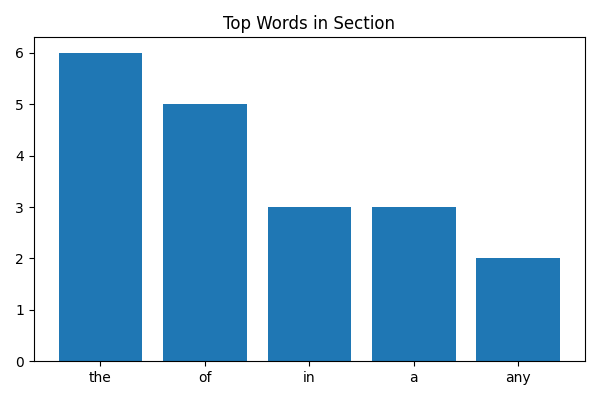
\includegraphics[width=0.8\textwidth]{D:\projects\mp 2 rag\autonomous rag\outputs\visual_6e4fde7278b041708d30c1c9e01c4abf.png}
\end{figure}
\section{10. Simple cognitive sets, selective}
Here's a summary of the section in clear and simple terms:

The author is discussing a new theory about how our brains learn and recognize things. This theory can explain how we learn to recognize different classes of things and remember them. However, it has limitations when it comes to understanding relationships between things in space and time.

The author is comparing this new theory to existing theories of learning and behavior. While the new theory is still not as developed as some of the other theories, it has some advantages. Specifically, it can predict how we learn and recognize things based on just six simple physical parameters, such as the number of connections between brain cells and the strength of those connections.

This is an improvement over other theories because it is based on measurable physical variables, which makes it more straightforward and testable. The author claims that this new theory is more concise, verifiable, and powerful in explaining how we learn and behave compared to other theories.

Further reading: https://www.semanticscholar.org/search?q=10.%20Simple%20cognitive%20sets,%20selective
\begin{figure}[h]
\centering
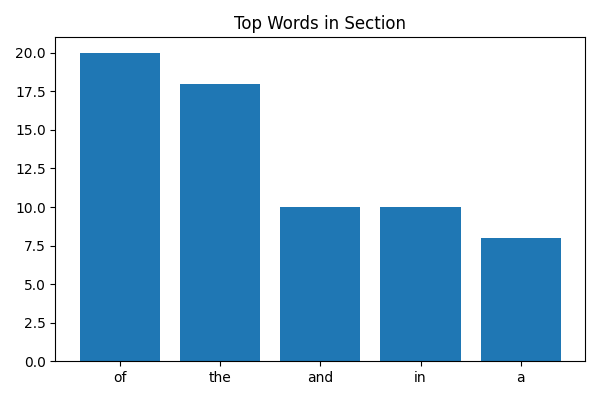
\includegraphics[width=0.8\textwidth]{D:\projects\mp 2 rag\autonomous rag\outputs\visual_2c210036a2644241b7ff96e690714f09.png}
\end{figure}
\section{1. Parsimony. Essentially}
Here's a simple summary:

The system uses basic ideas and rules from physical and biological science. The only new idea we need to add is a concept called "V", which represents the "value" of a connection between things. This "V" has to follow certain rules and is thought to have a physical basis that can be measured.

Further reading: https://arxiv.org/search/?query=1.+Parsimony.+Essentially&searchtype=all
\begin{figure}[h]
\centering
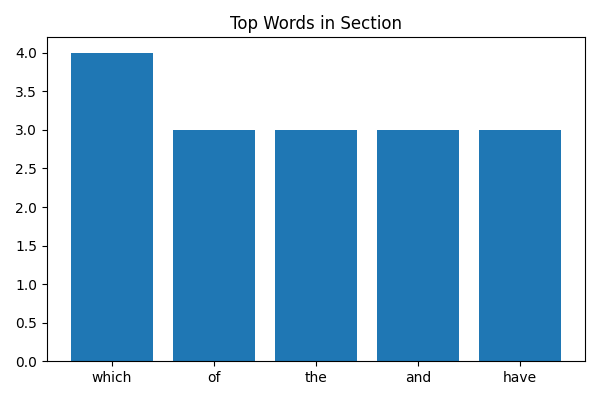
\includegraphics[width=0.8\textwidth]{D:\projects\mp 2 rag\autonomous rag\outputs\visual_f847a3f1571240c39e761452c6271643.png}
\end{figure}
\section{2. Verifiability.}
Here's a simple summary:

Old learning theories tried to predict how people would behave in new situations by measuring how they behaved in other situations. This is like trying to fit a curve to some data points and then hoping that the same curve will work for new data points. This approach has some problems. It's hard to justify why the same rules should apply in a new situation, and if the rules don't work, you can just change them to make them fit again. This means that these theories are hard to prove or disprove, and many psychologists think it's not worth trying to disprove them because they can always be adjusted to fit the data.

Further reading: https://arxiv.org/search/?query=2.+Verifiability.&searchtype=all
\begin{figure}[h]
\centering
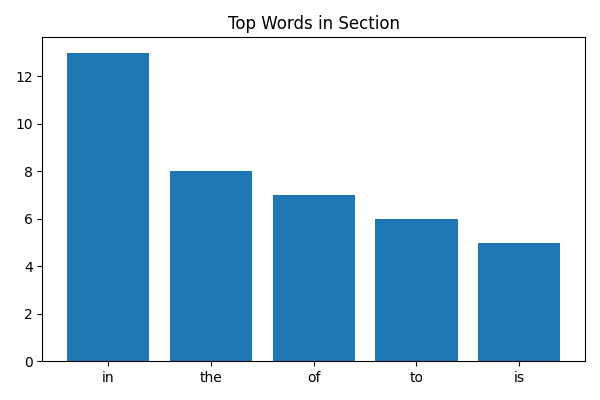
\includegraphics[width=0.8\textwidth]{D:\projects\mp 2 rag\autonomous rag\outputs\visual_14f0ac2870ce4ae592496a55a6fbfec6.png}
\end{figure}
\section{THE PERCEPTRON}
Here's a summary of the section in simple terms:

Some scientists think that choosing a theoretical model is just a matter of personal preference, and that any model can be made to fit the data. But this isn't true when the variables in the model can be measured independently. In a good theory, if the data doesn't fit, it means either the theory or the measurements are wrong. If a theory passes many tests, we can be more confident that it's correct and applies to many situations. This is better than a theory that has to be adjusted to fit each new situation.

Further reading: https://arxiv.org/search/?query=THE+PERCEPTRON&searchtype=all
\begin{figure}[h]
\centering
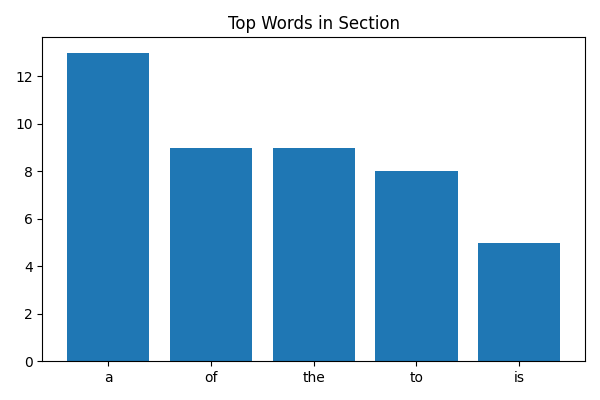
\includegraphics[width=0.8\textwidth]{D:\projects\mp 2 rag\autonomous rag\outputs\visual_6ad5dd8e34c049c0acaa1486a8988234.png}
\end{figure}
\section{3. Explanatory power and generality.}
Here's a summary of the section in clear, simple terms:

The theory being discussed is special because it's based on basic physical principles, which means it can be applied to any living thing or machine that processes information. This makes it very powerful and flexible. Other theories of learning are limited because they're based on specific examples or situations, and they become less accurate when applied to different situations. This new theory, on the other hand, remains precise and accurate even when applied to different situations.

The theory is also unique because it connects the physical workings of the brain to behavior and learning. This means that scientists can use the theory to predict how someone will learn or behave based on their brain's physical properties, and vice versa. This connection between brain and behavior is a major breakthrough.

The goal of this research is to understand the fundamental laws that govern how all information-handling systems, including humans and machines, work. By studying simple systems like the perceptron, scientists hope to gain insights that can be applied to more complex systems, ultimately leading to a deeper understanding of how we think and learn.

Further reading: https://www.semanticscholar.org/search?q=3.%20Explanatory%20power%20and%20generality.
\begin{figure}[h]
\centering
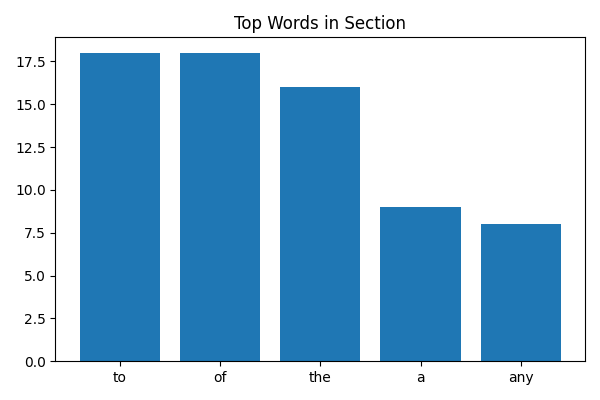
\includegraphics[width=0.8\textwidth]{D:\projects\mp 2 rag\autonomous rag\outputs\visual_7724ba0ef92347178f56b925b695ed90.png}
\end{figure}
\section{1. ASHBY, W. R. Design for a brain. New}
This section appears to be a citation or reference to a book. Here's a simple summary:

The book was published in New York by Wiley in 1952.

Further reading: https://arxiv.org/search/?query=1.+ASHBY,+W.+R.+Design+for+a+brain.+New&searchtype=all
\begin{figure}[h]
\centering
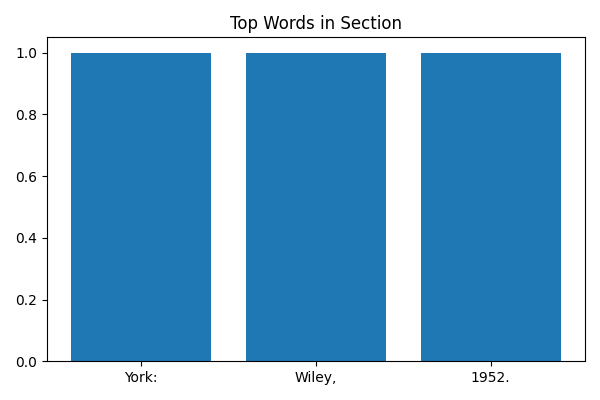
\includegraphics[width=0.8\textwidth]{D:\projects\mp 2 rag\autonomous rag\outputs\visual_9de30803ea4e4afcb49c35b870ca5fae.png}
\end{figure}
\section{2. CULBERTSON, J. T. Consciousness and be-}
I apologize, but the section you provided appears to be a citation or reference, rather than a passage of text that can be summarized. It lists a publication titled "havior" (which is likely a typo and should be "Behavior") published in Dubuque, Iowa by Wm. C. Brown in 1950. If you could provide more context or the actual text you'd like me to summarize, I'd be happy to help!

Further reading: https://www.semanticscholar.org/search?q=2.%20CULBERTSON,%20J.%20T.%20Consciousness%20and%20be-
\begin{figure}[h]
\centering
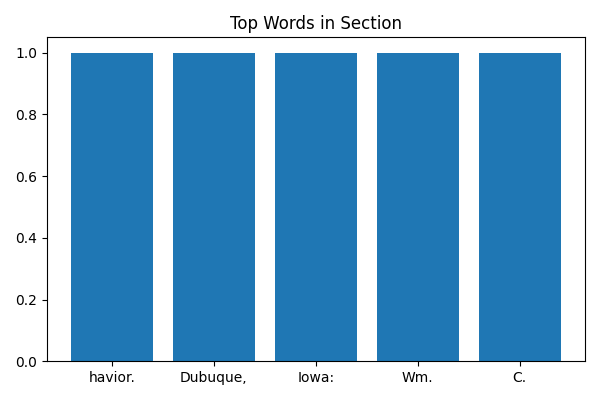
\includegraphics[width=0.8\textwidth]{D:\projects\mp 2 rag\autonomous rag\outputs\visual_4405cadfe8be4763bec57c8ae6e54e68.png}
\end{figure}
\section{3. CULBERTSON, J. T. Some uneconomical}
Here is a summary of the section in clear, simple terms:

This is a reference to a book chapter about robots, written by an unknown author. The chapter is part of a book called "Automata Studies", edited by C.E. Shannon and J. McCarthy, and published by Princeton University Press.

Further reading: https://arxiv.org/search/?query=3.+CULBERTSON,+J.+T.+Some+uneconomical&searchtype=all
\begin{figure}[h]
\centering
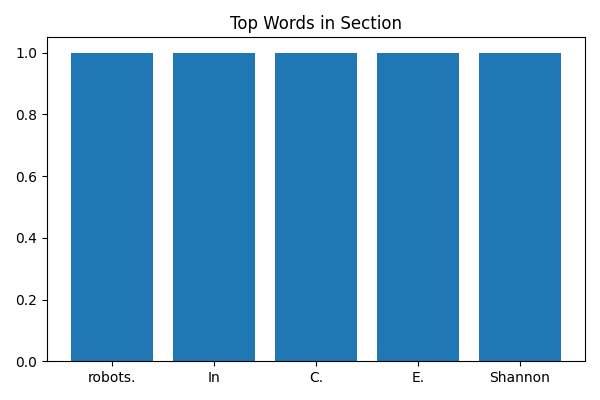
\includegraphics[width=0.8\textwidth]{D:\projects\mp 2 rag\autonomous rag\outputs\visual_b9ec093fcba24cf696c9cc07449d28ed.png}
\end{figure}
\section{4. ECCLES, J. C. The neurophysiological}
It seems like you only provided a partial sentence or title. Could you please provide more context or information about what you would like me to summarize?

From what you've provided, it appears to be a book title: "Basis of Mind" published by Clarendon in Oxford. If you could provide more context or information about the book's content, I'd be happy to help you summarize it in clear and simple terms.

Further reading: https://www.semanticscholar.org/search?q=4.%20ECCLES,%20J.%20C.%20The%20neurophysiological
\begin{figure}[h]
\centering
\includegraphics[width=0.8\textwidth]{D:\projects\mp 2 rag\autonomous rag\outputs\visual_3aaa82fd0aed40c7bb5b49b2a4d6fe02.png}
\end{figure}
\section{1953.
5. GOLDSTEIN, K. Human nature in the}
This section appears to be a reference to a book. Here's a simple summary:

The book is titled "Light of Psychopathology" and was published in 1940 by Harvard University Press in Cambridge.

Further reading: https://www.semanticscholar.org/search?q=1953.
5.%20GOLDSTEIN,%20K.%20Human%20nature%20in%20the
\begin{figure}[h]
\centering
\includegraphics[width=0.8\textwidth]{D:\projects\mp 2 rag\autonomous rag\outputs\visual_dbc2aa50a5d14b7890e525a3c2f8ef89.png}
\end{figure}
\section{6. HAYEK, F. A.}
Here is a summary of the section in clear, simple terms:

The book "The Sensory Order" was published in 1952 by the University of Chicago Press.

Further reading: https://www.semanticscholar.org/search?q=6.%20HAYEK,%20F.%20A.
\begin{figure}[h]
\centering
\includegraphics[width=0.8\textwidth]{D:\projects\mp 2 rag\autonomous rag\outputs\visual_a60a85dc2df94b138b9f2c58e33b0f54.png}
\end{figure}
\section{7. HEBB, D. O.}
This is a book title and publication information. Here's a simple summary:

The book is called "The Organization of Behavior" and it was published in New York by Wiley in 1949.

Further reading: https://scholar.google.com/scholar?q=7.+HEBB,+D.+O.
\begin{figure}[h]
\centering
\includegraphics[width=0.8\textwidth]{D:\projects\mp 2 rag\autonomous rag\outputs\visual_7afab7ae0a2b46d4bee9859adddb6706.png}
\end{figure}
\section{8. KLEENE, S. C. Representation of events}
Here is a summary of the section in clear, simple terms:

This is a reference to a chapter in a book called "Automata Studies" edited by C.E. Shannon and J. McCarthy, published in 1956 by Princeton University Press. The chapter is about nerve nets and finite automata, and it's on pages 3-41 of the book.

Further reading: https://www.semanticscholar.org/search?q=8.%20KLEENE,%20S.%20C.%20Representation%20of%20events
\begin{figure}[h]
\centering
\includegraphics[width=0.8\textwidth]{D:\projects\mp 2 rag\autonomous rag\outputs\visual_021bee705504464cb65386db1d4c98fe.png}
\end{figure}
\section{9. KOHLER, W. Relational determination}
This is a reference to a chapter in a book. Here's a simple summary:

The chapter is about how our brain works when we perceive things. It's part of a book called "Cerebral mechanisms in behavior" edited by L.A. Jeffress, published in 1951 by Wiley in New York. The chapter is on pages 200-243.

Further reading: https://www.semanticscholar.org/search?q=9.%20KOHLER,%20W.%20Relational%20determination
\begin{figure}[h]
\centering
\includegraphics[width=0.8\textwidth]{D:\projects\mp 2 rag\autonomous rag\outputs\visual_575f7d811acf4ce6b22165f13bae560b.png}
\end{figure}
\section{10. McCuLLOCH, W. S. Why the mind is in}
This is a reference to a chapter in a book. Here's a simple summary:

The chapter is about the brain and its role in behavior. It's part of a book called "Cerebral Mechanisms in Behavior" edited by L.A. Jeffress, published in 1951 by Wiley in New York. The chapter is on pages 42-111.

Further reading: https://arxiv.org/search/?query=10.+McCuLLOCH,+W.+S.+Why+the+mind+is+in&searchtype=all
\begin{figure}[h]
\centering
\includegraphics[width=0.8\textwidth]{D:\projects\mp 2 rag\autonomous rag\outputs\visual_271979885d9f42408ddc6770493aa884.png}
\end{figure}
\section{11. MCCULLOCH, W. S., & PITTS, W.}
Here is a summary of the section in clear, simple terms:

The section is referring to a scientific paper published in 1943 in a journal called "Bulletin of Mathematical Biophysics". The paper is about a mathematical system that tries to understand how the brain works and how it processes information.

Further reading: https://www.semanticscholar.org/search?q=11.%20MCCULLOCH,%20W.%20S.,%20&%20PITTS,%20W.
\begin{figure}[h]
\centering
\includegraphics[width=0.8\textwidth]{D:\projects\mp 2 rag\autonomous rag\outputs\visual_5e4948eea3fb457987883d4ac1c470dd.png}
\end{figure}
\section{12. MILNER, P. M. The cell assembly:}
It seems like you provided a very short section!

From what you provided, it appears to be a reference to a psychology article or paper. Here's a simple summary:

* The title of the paper is "Mark II"
* It was published in the "Psychological Review" journal
* The publication year is 1957
* The volume number is 64
* The page number is 242 (and possibly others, but the exact range is not specified)

Further reading: https://arxiv.org/search/?query=12.+MILNER,+P.+M.+The+cell+assembly:&searchtype=all
\begin{figure}[h]
\centering
\includegraphics[width=0.8\textwidth]{D:\projects\mp 2 rag\autonomous rag\outputs\visual_71562d640c974c928f8a9bba56576a6d.png}
\end{figure}
\section{252.
13. MINSKY, M. L. Some universal elements}
Here is a summary of the section in clear, simple terms:

This is a reference to a chapter in a book called "Automata Studies" edited by C.E. Shannon and J. McCarthy, published in 1956 by Princeton University Press. The chapter is about finite automata and is on pages 117-128.

Further reading: https://www.semanticscholar.org/search?q=252.
13.%20MINSKY,%20M.%20L.%20Some%20universal%20elements
\begin{figure}[h]
\centering
\includegraphics[width=0.8\textwidth]{D:\projects\mp 2 rag\autonomous rag\outputs\visual_c1615ef7bc784354a1406200e4972a2a.png}
\end{figure}
\section{14. RASHEVSKY, N. Mathematical biophysics.}
This is a book citation. Here's what it means in simple terms:

* The book was published in Chicago.
* The publisher is the University of Chicago Press.
* The book was published in 1938.

Further reading: https://arxiv.org/search/?query=14.+RASHEVSKY,+N.+Mathematical+biophysics.&searchtype=all
\begin{figure}[h]
\centering
\includegraphics[width=0.8\textwidth]{D:\projects\mp 2 rag\autonomous rag\outputs\visual_466428a325c14db2a40e4a636e473d3f.png}
\end{figure}
\section{15. ROSENBLATT, F.}
Here is a summary of the section in clear, simple terms:

The title refers to a research report written in 1958 by the Cornell Aeronautical Laboratory. The report is about a concept called the "perceptron", which is a theory that explains how cognitive systems (like our brains) can separate and distinguish between different things based on statistical patterns.

Further reading: https://arxiv.org/search/?query=15.+ROSENBLATT,+F.&searchtype=all
\begin{figure}[h]
\centering
\includegraphics[width=0.8\textwidth]{D:\projects\mp 2 rag\autonomous rag\outputs\visual_6a90ac98b5fb4d5baf7662798b8637a1.png}
\end{figure}
\section{16. UTTLEY, A. M. Conditional probability}
Here is a summary of the section in clear, simple terms:

This is a chapter in a book called "Automata Studies" edited by C.E. Shannon and J. McCarthy, published in 1956 by Princeton University Press. The chapter is about machines and conditioned reflexes, and it spans pages 253-275 of the book.

Further reading: https://www.semanticscholar.org/search?q=16.%20UTTLEY,%20A.%20M.%20Conditional%20probability
\begin{figure}[h]
\centering
\includegraphics[width=0.8\textwidth]{D:\projects\mp 2 rag\autonomous rag\outputs\visual_281aa7a24ebf4433b9ae74793530a8e0.png}
\end{figure}
\section{17. VON NEUMANN, J.}
Here is a summary of the section in clear, simple terms:

This is a chapter in a book called "Cerebral Mechanisms in Behavior" edited by L.A. Jeffress and published in 1951 by Wiley in New York. The chapter is titled "The General and Logical Theory of Automata" and it spans pages 1-41.

Further reading: https://www.semanticscholar.org/search?q=17.%20VON%20NEUMANN,%20J.
\begin{figure}[h]
\centering
\includegraphics[width=0.8\textwidth]{D:\projects\mp 2 rag\autonomous rag\outputs\visual_fdb6d0949707449c86652ad4b4d36aab.png}
\end{figure}
\section{18. VON NEUMANN, J.}
Here is a summary of the section in clear, simple terms:

This is a reference to a chapter in a book called "Automata Studies" edited by C.E. Shannon and J. McCarthy, published in 1956 by Princeton University Press. The chapter is about using probability to create reliable systems from unreliable parts.

Further reading: https://scholar.google.com/scholar?q=18.+VON+NEUMANN,+J.
\begin{figure}[h]
\centering
\includegraphics[width=0.8\textwidth]{D:\projects\mp 2 rag\autonomous rag\outputs\visual_e471c9298acd462096fb99035e0c8a12.png}
\end{figure}
\end{document}